\documentclass[a4paper,10pt,twocolumn]{myjarticle2}

\usepackage[dvipdfmx]{graphicx}
\usepackage{url}

\input{header}

\renewcommand{\figurename}{Figure}
\renewcommand{\tablename}{Table}
\renewcommand{\refname}{References}

\pagestyle{empty}

\setlength{\topmargin}{6mm}
\setlength{\oddsidemargin}{-4mm}
\setlength{\evensidemargin}{-4mm}
\setlength{\textwidth}{170mm}
\setlength{\headsep}{0pt}
\setlength{\headheight}{0pt}
\setlength{\textheight}{235mm}
\setlength{\columnsep}{5mm}

\newcommand{\Hraw}{H_{\mathrm{raw}}}
\newcommand{\Hstar}{H^{\ast}}

\begin{document}
\twocolumn[%
\vspace{-20mm}
\begin{center}
{\LARGE\bf Membership Specification and Sensitivity Reporting for
Fuzzy-Entropy-Based LLM Emotion Scoring}
\vspace{2mm}\par\noindent
{\large
$\bigcirc$ Naruki Shirahama$^{1}$, Yuma Yoshimoto$^{2}$, Naofumi Nakaya$^{3}$,\\
Junji Nishino$^{4}$, and Satoshi Watanabe$^{5}$}
\vspace{2mm}\par\noindent
{\small
$^{1}$Shimonoseki City University, Shimonoseki, Yamaguchi, Japan\\
$^{2}$NIT (KOSEN), Kitakyushu College, Kitakyushu, Fukuoka, Japan\\
$^{3}$Juntendo University, Urayasu, Chiba, Japan\\
$^{4}$Tamagawa University, Machida, Tokyo, Japan\\
$^{5}$Shizuoka Institute of Science and Technology, Fukuroi, Shizuoka, Japan\\
Contact: \url{nshirahama@ieee.org}}
\vspace{2mm}\par\noindent
\begin{minipage}{150mm}
{\small
{\bf Abstract:}
Fuzzy entropy has been used as an ambiguity descriptor for continuous emotion
scores produced by large language models. However, the resulting entropy value
is not determined by the score alone; it also depends on the
membership-function specification used to map a 0--100 score into Low, Medium,
and High fuzzy memberships. This paper proposes a membership
specification card and a score-axis sensitivity-reporting protocol for
fuzzy-entropy-based LLM emotion scoring. The proposed report records the score
range, score grid, labels, breakpoints, membership family, smoothness, endpoint
behavior, entropy formula, family-specific normalization constant, and version
identifier. Using three score-axis membership families--piecewise linear,
Zadeh-type S/Z/pi, and sigmoid-composed S/Z/pi--we illustrate how normalized
entropy-response curves $\Hstar(x)$ and family-pair sensitivity summaries can
be reported without introducing model rankings, persona-temperature analyses,
or benchmark-positioning results. The aim is not to select a universally
correct membership function, but to make fuzzy-entropy reports reproducible and
auditable.
\par\noindent
}
\end{minipage} \par\noindent
\end{center}
]

\section{Introduction}

Continuous emotion scores produced by large language models (LLMs) are often
reported on a bounded scale, for example from 0 to 100. Fuzzy-set methods offer
a convenient way to describe such scores using linguistic memberships such as
Low, Medium, and High. A scalar fuzzy entropy can then be used as an ambiguity
descriptor: scores near a single dominant label have low entropy, while scores
near transitions among labels have higher entropy. Prior EQ-Fuzzy work used
fuzzy entropy as one LLM emotion-scoring descriptor [5]; this paper uses that
context only as motivation for reproducible reporting.

This descriptor is useful only when its membership specification is visible.
A score value does not determine its fuzzy entropy by itself. The entropy also
depends on the score range, breakpoints, membership-function family,
smoothness, endpoint behavior, and normalization convention. Two studies can
therefore use the same LLM score and the same entropy equation but report
different entropy values because their membership functions differ.

This paper is a methodological foundation for EQ-Fuzzy rather than a downstream
evaluation paper. Later EQ-Fuzzy work may use fuzzy entropy in human-alignment
analysis, factorial analysis, benchmark-positioning studies, or
annotation-support workflows. Those uses require that the descriptor itself be
specified before downstream interpretations begin. The present paper therefore
defines a reusable reporting unit for the descriptor and leaves downstream
evaluation results outside its scope.

The contribution is intentionally narrow. This paper does not evaluate which
LLM is best, rank providers, analyze persona-temperature effects, provide
human-grounded multilingual validation, or position EQ-Fuzzy against existing
benchmarks. It specifies what should be reported when fuzzy entropy is used as
a score-axis descriptor.

\section{Membership-Dependent Fuzzy Entropy}

Let $x \in [0,100]$ be a continuous emotion score. A membership specification
maps $x$ to three membership degrees
$\mu_L(x), \mu_M(x), \mu_H(x) \in [0,1]$ for Low, Medium, and High. In the
generated artifacts used here, the score-level descriptor is a Shannon-type
membership-overlap entropy [4],
\begin{equation}
\Hraw(x)=-\sum_{\ell \in \{L,M,H\}}\mu_\ell(x)\log_2\mu_\ell(x),
\end{equation}
where $0\log_2 0:=0$. For comparison across membership families, we report
\begin{equation}
\Hstar(x) = \Hraw(x) / H_{\max},
\end{equation}
where $H_{\max}$ is family-specific and is estimated on the documented dense
score grid. In the present artifact, the documented grid is
$0, 0.1, \ldots, 100.0$.

The membership values in Eq. (1) are not probabilities over labels. They are
grades of membership assigned by the chosen fuzzy partition of the 0--100
score axis. This distinction matters because the membership functions are part
of the measurement specification. A score of 25, for example, may be crisp
under one specification and transition-like under another. The entropy value is
therefore a descriptor of the pair consisting of the score and the documented
membership specification.

The dependence on membership functions is not incidental. Zadeh's fuzzy sets
are defined through membership grades over a universe of discourse [1]. The
De Luca--Termini formulation is part of the fuzzy-entropy literature [2], but
the concrete descriptor reported here is the membership-overlap entropy in
Eq. (1). Recent FSS discussion of membership functions also emphasizes that
values of the universe and the shape of the membership function jointly affect
interpretation [3]. For LLM emotion scoring, this means that an entropy number
should be read as ``entropy under a documented membership specification.''

The normalization constant $H_{\max}$ also belongs to the specification. It is
not a universal constant shared by all possible membership families. In this
paper, each family receives its own $H_{\max}$ estimated over the same dense
0--100 grid. The normalized response $\Hstar(x)$ is then a family-internal
scale for comparing where that family regards the score axis as more or less
ambiguous. Family-pair comparisons are reported separately as sensitivity
summaries rather than treated as model effects.

\section{Membership-Function Design Space}

The three families used in this proceedings paper are not proposed as the only
possible choices. They are representative design points for documenting how a
0--100 score axis is partitioned into Low, Medium, and High memberships. The
point is to make the design choice explicit and auditable.

The legacy linear family uses piecewise-linear low, medium, and high
memberships. This design is easy to inspect: transition intervals and peak
regions can be read directly from the breakpoints. Its limitation is that the
membership curves are only $C^0$ continuous and become nonsmooth at transition
points. Such nonsmoothness is not necessarily wrong, but it should be reported
because entropy-response curves inherit these local geometric choices.

The Zadeh S/Z/pi family smooths local transitions under the same semantic
breakpoint structure. S-shaped and Z-shaped functions make the Low and High
edges smoother, while the pi-like Medium membership summarizes a central band.
This design keeps the linguistic labels and score range stable but changes how
rapidly a score moves from one membership region to another.

The sigmoid-composed S/Z/pi family documents an additional score-axis warping
step before S/Z/pi mapping. In practical terms, the near-transition and
far-from-transition behavior can change smoothly while endpoint behavior is
handled explicitly. This is useful when the analyst wants smooth transitions
but still wants to state how exact endpoints and clipped interior values are
treated.

These three families align with the broader membership-function design issues
discussed by Umano [3]. Triangular and trapezoidal memberships can be
continuous and interpretable but nonsmooth. S/Z/pi functions smooth local
transitions. Sigmoid plus S-function composition can make near and far
score-axis behavior change smoothly. None of these observations implies that
the sigmoid-composed family is uniquely correct. They show why a report should
state the family, smoothness, and endpoint convention rather than leaving them
implicit.

\section{Complete Membership Specification Card}

Table 1 gives the complete membership specification card recommended for
score-axis fuzzy-entropy reports. It records fields that are often treated as
implementation detail but are necessary for reproducible interpretation.

\begin{table}
\centering
\caption{Complete membership specification card fields.}
\label{tab:complete-card}
\footnotesize
\setlength{\tabcolsep}{2pt}
\begin{tabular}{|p{23mm}|p{46mm}|}
\hline
Field & Required content \\
\hline
Score range & Closed interval for the score axis, here $[0,100]$. \\
\hline
Score grid & Dense grid used for response and $H_{\max}$ estimation. \\
\hline
Labels & Linguistic labels, here Low, Medium, and High. \\
\hline
Breakpoints & Label-transition and central-region score breakpoints. \\
\hline
Family ID & Versioned membership-function family identifier. \\
\hline
Smoothness & Continuity class or documented smoothness convention. \\
\hline
Endpoint behavior & Exact, clipped, or asymptotic endpoint handling. \\
\hline
Entropy formula & Equation for $\Hraw(x)$ and zero-term convention. \\
\hline
Normalization & Family-specific $H_{\max}$ and estimation grid. \\
\hline
Versioning & Artifact ID, config hash, and generation script version. \\
\hline
\end{tabular}
\end{table}

Table 2 shows the family-specific part of the card for the three artifacts used
in this paper. The exact version identifiers and configuration hashes are
retained in the machine-readable artifact; the manuscript uses short aliases to
keep the proceedings table readable.

\begin{table}
\centering
\caption{Family-specific fields in the membership specification card.}
\label{tab:family-card}
\footnotesize
\setlength{\tabcolsep}{2pt}
\begin{tabular}{|p{18mm}|p{16mm}|p{20mm}|p{10mm}|}
\hline
Family & Smoothness & Endpoint handling & $H_{\max}$ \\
\hline
linear & $C^0$ piecewise & exact endpoints & 1.0577 \\
\hline
Zadeh S/Z/pi & $C^1$ quadratic & exact endpoints & 1.0524 \\
\hline
sigmoid S/Z/pi & smooth transition & clipped interior values & 1.0184 \\
\hline
\end{tabular}
\end{table}

The card separates stable semantic choices from implementation choices. Score
range, labels, and breakpoints define what the score axis means. Family ID,
smoothness, and endpoint behavior define how membership degrees are assigned.
Entropy equation and normalization define how the membership vector is reduced
to a scalar descriptor. Versioning ties the prose report to reproducible
artifacts.

\section{Entropy-Response and Sensitivity Reporting}

Figure 1 illustrates the primary score-axis report. The upper panels show Low,
Medium, and High memberships over the score axis for three membership
families. The lower panel shows the corresponding normalized entropy-response
curves $\Hstar(x)$. The figure is deliberately score-axis-only: it contains no
model, provider, persona, temperature, benchmark, language-drift, or
target-shift results.

\begin{figure}
\centering
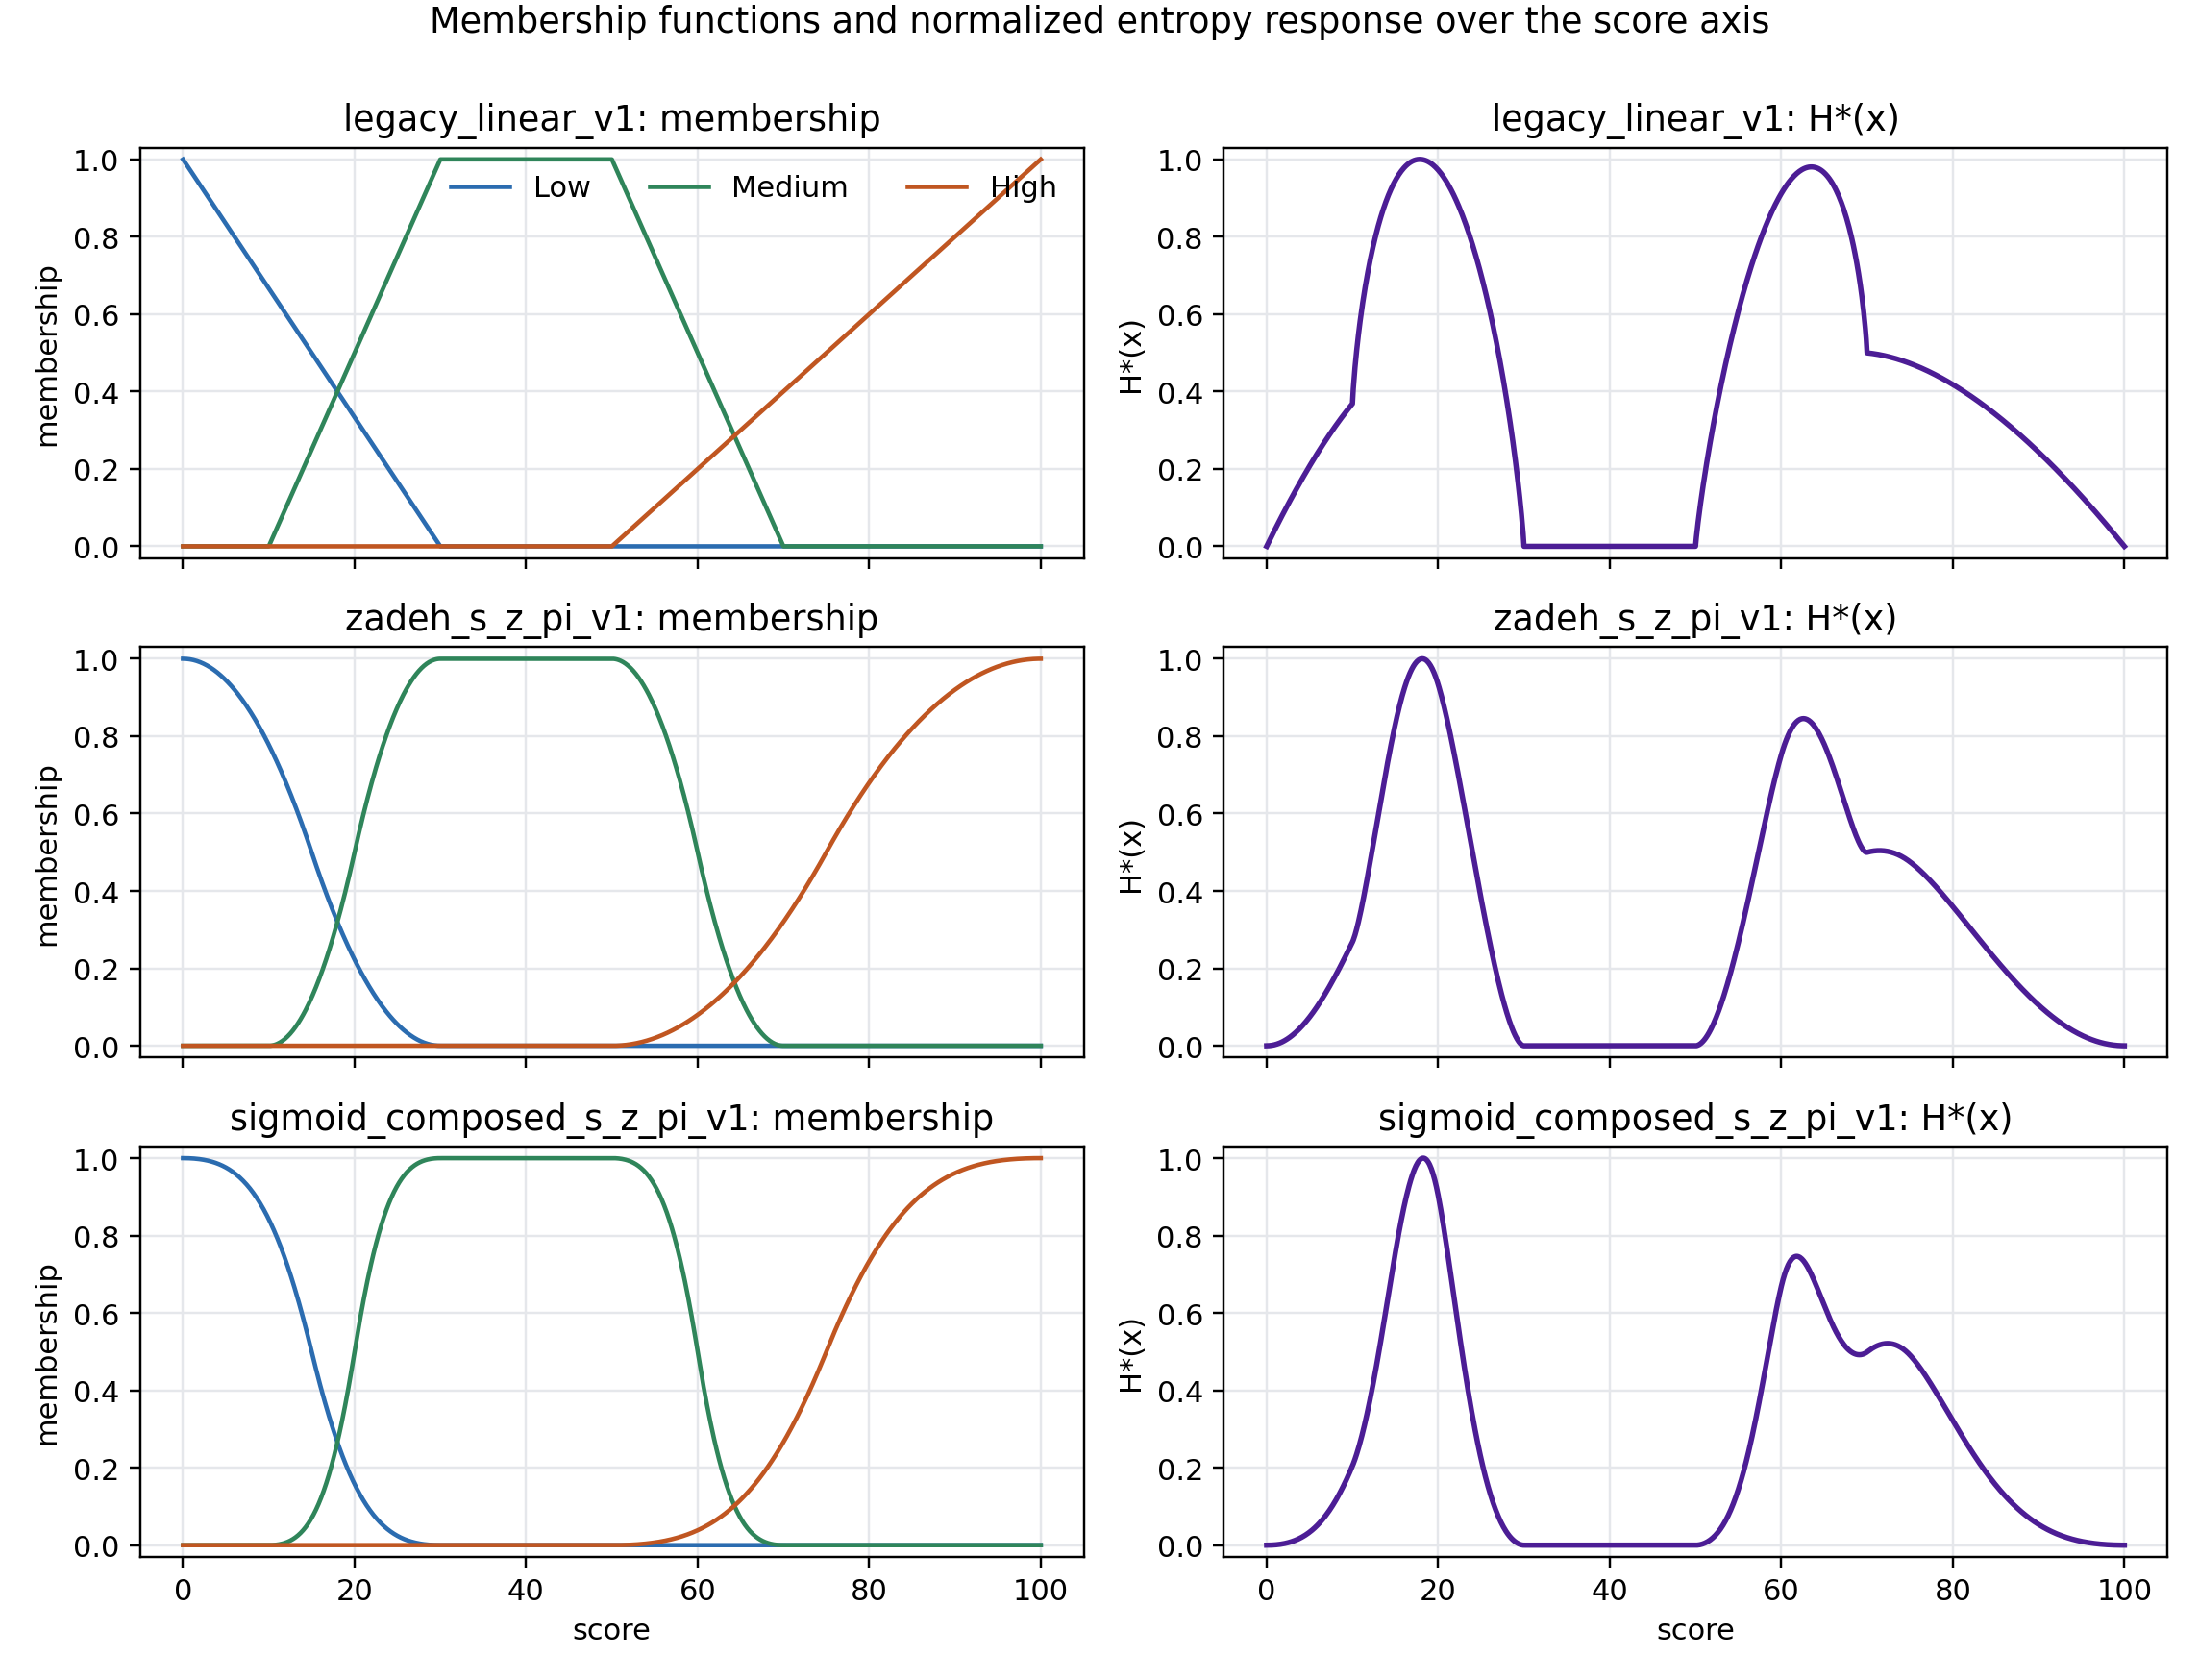
\includegraphics[width=\linewidth]{figures/figure1_membership_and_entropy_response.png}
\caption{Score-axis-only membership functions and normalized entropy-response
curves. The figure reports membership-family behavior over the 0--100 score
axis only and contains no model, provider, persona, temperature, benchmark, or
target-shift results.}
\label{fig:response}
\end{figure}

A minimal sensitivity report compares unordered family pairs over the same
score grid. Table 3 shows that the largest absolute differences in $\Hstar(x)$
occur in the Low--Medium transition region. These values are not model effects.
They are score-axis sensitivity summaries under alternative membership
specifications.

\begin{table}
\centering
\caption{Score-axis sensitivity summary over the documented 0--100 grid.}
\label{tab:sensitivity}
\footnotesize
\setlength{\tabcolsep}{2pt}
\begin{tabular}{|p{23mm}|p{11mm}|p{12mm}|p{18mm}|}
\hline
Pair & Max $|\Delta\Hstar|$ & Mean $|\Delta\Hstar|$ & max region \\
\hline
linear--Zadeh S/Z/pi & 0.343 & 0.110 & Low--Medium \\
\hline
linear--sigmoid-composed & 0.481 & 0.158 & Low--Medium \\
\hline
Zadeh S/Z/pi--sigmoid-composed & 0.167 & 0.048 & Low--Medium \\
\hline
\end{tabular}
\end{table}

The sensitivity values should be read before downstream evaluation results are
interpreted. If two membership families give substantially different
entropy-response curves near a transition region, a downstream entropy
comparison in that region should be reported with that caveat. If the
sensitivity is small for the relevant score region, the chosen family is less
likely to dominate interpretation. In both cases, the sensitivity report
protects the analysis from treating a specification choice as a model property.

The curve itself should also be read as a response surface over the score axis,
not as a histogram of observed outputs. Peaks in $\Hstar(x)$ indicate score
regions where the specified membership partition treats the score as highly
ambiguous among labels. Flat or near-zero regions indicate scores that the same
partition treats as close to crisp. These statements are properties of the
membership specification. They do not imply that any model produced many or few
scores in those regions.

This distinction is useful for experimental design. Before collecting or
analyzing downstream LLM outputs, a researcher can inspect the score-axis
response and ask whether the intended interpretation is plausible. If the
membership family creates a sharp entropy peak at a score region that will be
central to the later experiment, that later report should include the
sensitivity caveat. If the downstream score region is far from a transition,
the family choice may be less influential. In either case, the membership
specification is reviewed before it becomes entangled with model behavior.

The family-pair summaries in Table 3 are deliberately simple. The maximum
absolute difference identifies the largest local disagreement between two
families, while the mean absolute difference gives a coarse global summary over
the documented grid. The transition-region label helps readers locate the
largest disagreement without implying a downstream cause. A longer report could
add integrated differences or region-specific summaries, but the compact table
is sufficient for a proceedings-level reproducibility check.

The minimum reporting checklist is: (i) score range and grid resolution;
(ii) labels and breakpoints; (iii) family ID, smoothness, and endpoint
convention; (iv) entropy equation and family-specific $H_{\max}$; and
(v) score-axis sensitivity against at least one plausible alternative family.
This checklist is intentionally smaller than a full experiment table. It is
meant to make the descriptor auditable before any downstream LLM comparison is
interpreted.

\section{Reproducibility and Artifact Discipline}

Figure 2 shows the intended reporting workflow. A 0--100 score is first mapped
through a documented membership family to Low, Medium, and High memberships.
Those memberships are reduced to $\Hraw(x)$, normalized to $\Hstar(x)$, and
then checked by score-axis sensitivity analysis before downstream use.

\begin{figure}
\centering
\footnotesize
\setlength{\tabcolsep}{1pt}
\begin{tabular}{c}
\fbox{\parbox{60mm}{\centering 0--100 score}}\\[1mm]
$\downarrow$\\[-1mm]
\fbox{\parbox{60mm}{\centering documented membership family}}\\[1mm]
$\downarrow$\\[-1mm]
\fbox{\parbox{60mm}{\centering Low/Medium/High memberships}}\\[1mm]
$\downarrow$\\[-1mm]
\fbox{\parbox{60mm}{\centering $\Hraw(x)$, then $\Hstar(x)$}}\\[1mm]
$\downarrow$\\[-1mm]
\fbox{\parbox{60mm}{\centering score-axis sensitivity report}}\\[1mm]
$\downarrow$\\[-1mm]
\fbox{\parbox{60mm}{\centering downstream evaluation, reported separately}}
\end{tabular}
\caption{Generic score-axis reporting workflow. The workflow contains no model
names, provider names, persona labels, temperature levels, benchmark names, or
human-alignment results.}
\label{fig:workflow}
\end{figure}

The generated artifact set supports this workflow. The configuration file
defines the score range, grid, family identifiers, breakpoints, and endpoint
conventions. The membership grid records Low, Medium, and High memberships on
the documented score axis. The entropy-response grid records $\Hraw(x)$ and
$\Hstar(x)$ for each family. The membership specification card and family
sensitivity matrix are exported both as machine-readable tables and LaTeX
tables. The figure summary and analysis summary record scope checks, generated
paths, family-specific $H_{\max}$ values, and the fact that the content is
score-axis-only.

The artifact filenames are retained for auditability. They include grid
exports for membership and entropy response, card exports in CSV and LaTeX
form, sensitivity-matrix exports in CSV and LaTeX form, and JSON summaries for
the figure and analysis. These artifacts are generated derivatives. This paper
does not use API calls, does not read raw JSONL outputs, and does not copy raw
experimental responses into the manuscript.

This discipline is important because fuzzy entropy can otherwise appear to be
a standalone scalar. The proposed report makes clear which parts are
mathematical definitions, which parts are membership-function design choices,
and which parts are generated score-axis summaries. Downstream studies can
then cite or reuse the reporting unit without importing paper-specific claims.

The artifact boundary also protects future revisions. A manuscript can revise
its prose, but the artifact ID and configuration hash state which membership
specification produced the figure and tables. If a later study changes
breakpoints, endpoint behavior, or the score grid, it should receive a new
card and sensitivity report rather than silently reusing the old descriptor
label. This is especially important when a descriptor is shared across multiple
papers: shared code is useful, but shared claims should not be smuggled through
unchanged filenames.

Finally, the artifact discipline makes negative scope statements verifiable.
The figure summary records that the figure contains no model names and no
persona or temperature labels. The analysis summary records that no API calls
were made and that no raw JSONL files were read or copied for this paper. These
statements are modest, but they are part of the audit trail: the FSS paper is a
membership-specification report, not an experimental result report.

\section{Discussion and Conclusion}

The proposed card does not identify a universally correct membership function.
In many LLM emotion-scoring settings, several membership families may be
defensible. The practical requirement is that the chosen family be specified
and that nearby plausible choices be sensitivity-checked. Without that record,
fuzzy entropy values can appear more self-contained than they really are.

The reporting unit supports later downstream evaluations by making the
descriptor layer explicit. Human-alignment studies, persona-temperature
factorial analyses, benchmark-positioning work, and annotation-support
workflows may all use fuzzy entropy, but they should not need to redefine the
membership specification each time. This paper provides that reporting
specification. It does not report results from those workstreams.

This paper reframes fuzzy entropy for LLM emotion scoring as a
specification-dependent descriptor. A reproducible report should state the
membership-function family, breakpoints, smoothness, endpoint handling,
entropy formula, family-specific normalization, versioning information, the
score-axis entropy response, and at least a minimal sensitivity summary. This
small discipline is intended to make future EQ-Fuzzy evaluations reproducible
and auditable without treating membership-function choices as downstream model
effects.

The practical recommendation is therefore simple. When fuzzy entropy is used
with bounded continuous emotion scores, the entropy value should not be
reported alone. It should be accompanied by the membership card, the
entropy-response curve, and at least one score-axis sensitivity comparison
against a plausible alternative family. That package is small enough to include
in a proceedings paper, but explicit enough to keep later evaluations from
depending on undocumented membership-function assumptions.

\vspace{1mm}
\noindent{\large\bf Acknowledgment}\par\noindent

This work is part of the EQ-Fuzzy research line. This work was partially
supported by JSPS Grants-in-Aid for Scientific Research (JSPS KAKENHI), Grant
Numbers 26K14983 and 24K13350. The present manuscript uses only generated
score-axis membership-specification artifacts and does not use API calls or raw
JSONL outputs.

\vspace{1mm}
\noindent{\large\bf References}\par\noindent
[1] L. A. Zadeh, ``Fuzzy sets,'' \emph{Information and Control}, vol. 8,
no. 3, pp. 338--353, 1965.
\par\noindent
[2] A. De Luca and S. Termini, ``A definition of a nonprobabilistic entropy in
the setting of fuzzy sets theory,'' \emph{Information and Control}, vol. 20,
no. 4, pp. 301--312, 1972.
\par\noindent
[3] M. Umano, ``Some considerations on membership functions of fuzzy sets,''
\emph{Proceedings of the Fuzzy System Symposium}, vol. 41, no. 0, pp. 70--74,
2025, \url{https://doi.org/10.14864/fss.41.0_70}.
\par\noindent
[4] C. E. Shannon, ``A mathematical theory of communication,'' \emph{Bell
System Technical Journal}, vol. 27, no. 3, pp. 379--423, 1948.
\par\noindent
[5] N. Shirahama, Y. Yoshimoto, N. Nakaya, and S. Watanabe, ``Mathematical
framework for characterizing emotional individuality in large language models:
Temperature control, fuzzy entropy, and persona-based diversity analysis,''
\emph{Mathematics}, vol. 14, no. 7, Art. no. 1224, 2026,
doi:10.3390/math14071224.

%%%%% Contact Information%%%%%
\vspace{1mm}
\noindent{\large\bf Contact Information}\par\noindent
\begin{tabular}{l}
Naruki Shirahama \\
Shimonoseki City University\\
E-mail: {\tt  nshirahama@ieee.org}
\end{tabular}

\end{document}
